\باب{پس نوشت}\شناخت{باب_پس_نوشت}
%typing complete
اب چونکہ میں توقع کرتا ہوں آپ کوانٹم میکانیات کو سمجھتے ہیں ہم \حوالہء{حصہ \num{1.2}} میں کیا گیا سوال دوبارہ اٹھاتے ہیں کوانٹم میکانیات کے نتائج سے کیا مطلن اغز کرنا چاہیئے مسئلہ کا جڑ تفاعل موج کے ساتھ وابستہ شماریتای مفہوم کی عدم تعینیت ہے۔ تفاعل \عددی{\ساے} یا کوانٹم حال کہنا بہتر ہوگا جو مثال کے طور پر چکرکار ہو سکتا ہے صرف ممکنہ نتائج کی شماریاتی تقسیم مہیا کرتا ہے اور کسی بھی پیمائش کا نتیجہ یکتا طور پر تعین نہیں کرتا اس سے ایک اہم سوال کھڑا ہوتا ہے کیا پیمائش سے قبل نظام یہ مخصوص خاصیت حقیقتاً رکھتا تھا جسے حقیقت پسند نقطہ نظر کہتے ہیں یا پیمائش کے عامل نے اس خاصیت کو جنم دیا جو تافعل موج کی شماریاتی پابندی کو مطمعن کرتا ہے۔ تقلید پسند نقطہ نظر یا ہم اس سوال کو ان بنیادوں پر رد کرتے ہیں کہ یہ سوال ایک فرضی سوال ہے انکاری نقطہ نظر۔

حقیقت پسند کے نقطہ نظر سے کوانٹم میکانیات ایک نا مکمل نظریہ ہے چونکہ کوانٹم میکانیات کی تمام فراہم کردہ معلومات یعنی اس کا تفاعل موج جانتے ہوئے آپ خواص تعین نہیں کر سکتے ہیں۔ ظاہر ہے ایسی صورت میں کوانٹم میکانیات سے باہر کوئی اور معلومات ہوگی جس کو \عددی{\ساے} کے ساتھ ملا کر طبعی حقائق کو مکلم طور پر بیان کرنا ممکن ہوگا۔

تقلید پسند نقطہ نظر اس سے بھی زیادہ سنگین سوالات کھڑے کرتا ہے چونکہ اگر پیمائشی عمل نظام کو ایک خاصیت اختیار کرنے پر مجبور کرتا ہو تب پیمائش ایک عجیب عمل ہوگا ساتھ ہی یہ جانتے ہوئے کہ ایک پیمائش کے فوراً بعد دوسری پیمائش وہی نتیجہ دیتی ہے ہمیں ماننا ہوگا کہ پیمائشی عمل تفاعل موج کو یوں منحداً کرتا ہے جو مساوات شروڈنگر کی تجویز کردہ ارتقا کے برعکس ہے۔

ان سب کی روشنی میں ہم دیکھ سکتے ہیں کہ نسل در نسل ماہرِ طبیعیات انکاری سوچ کے پیچھے پنا لینے پر مجبور کیوں ہوئے اور اپنے شاگردوں کو نصیحت کرتے رہے کہ نظریہ کے تصوراتی بنیادوں پر غور و فکر کر کے اپنا وقت ضائع نہ کریں۔
\حصہ{آئنسٹائن پوڈلسکیو روزن تضاد}
\سن{1935}میں آئنسٹائن پوڈلسکی اور روزن نے مل کر آئنسٹائن پوڈلسکی اور روزن تضاد پیش کیا جسکا مقصد خالصتاً نظریاتی بنیادوں پر یہ ثابت کرنا تھا کہ صرف حقیقت پسندانا نقطہ نظر درست ہوسکتا ہے۔ میں اس تضاد کی ایک سادہ روپ جو داؤد بام نے پیش کی پر تبصرہ کرتا ہوں۔ تادیلی پاے میزان کی ایک الیکٹران اور ایک پرٹون میں تحلیل پر غور کریں
\begin{align*}
	\pi^0\to e^{-}+e^{+}
\end{align*}
%
\begin{figure}
\centering
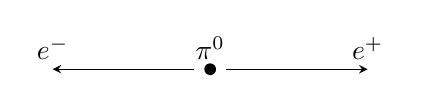
\begin{tikzpicture}
\draw[-stealth] (-0.2,0) -- (-2,0) node[above]{$e^{-}$};
\draw[-stealth] (0.2,0) -- (2,0) node[above]{$e^{+}$};
\draw[] (0,0) node[circle, inner sep=1.5pt, fill=black]{} node[above]{$\pi^{0}$};
\end{tikzpicture}
\caption{آئنشٹائن، پوڈلسکی و  روزن  تضاد کا بوہم انداز۔ساکن \عددی{\pi^0}  کا تنزل الیکٹران و  ضد الیکٹران  جوڑی میں ہوتا ہے۔}
\label{شکل_بکھراو_بوہم_تنزل}
\end{figure}

ساکن پائون کی صورت میں الیکٹران اور پروٹان ایک دوسرے کے مخالف رخ جائیں گے (شکل \حوالہ{شکل_بکھراو_بوہم_تنزل})۔ اب چونکہ پائون کا چکر صفر ہے لحاظہ زاویائی معیارِ حرکت کی بقا کے تحت یہ الیکٹران اور پوزیٹران یکتا تنظیم میں ہوں گے
\begin{align}
	\frac{1}{\sqrt{2}}(\uparrow_{-}\downarrow_{+}-\downarrow_{-}\uparrow_{+})
\end{align}
اگر دیکھا جائے کہ الیکٹران ہم میدان ہے تب پوزیٹران لاظماً خلافِ میدان ہوگا اور اسی طرح اگر الیکٹران خلاف میدان پایا جائے تب پوزیٹران ہم میدان ہوگا۔ کوانٹم میکانیات آپ کو یہ بتناے سے قاصر ہے کہ کس پایون تحویل میں آپ کو کونسی صورت حال ملے گی تاہم کوانٹم میکانیات یہ ضرور بتا سکتی ہے کہ ان پیمائش کا ایک دوسرے کے ساتھ تعلق ہوگا اور اوسطاً نصف وقت ایک قسم اور نصف وقت دوسری قسم کی جوڑیاں پیدا ہوں گے۔ اب فرض کریں ہم ان الیکٹران اور پوزیٹران کو ایک عملی تجربہ کے لیئے دس میٹر تک جانے دیں یا اصولاً دس نوری سال تک جانے دیں اور اس کے بعد الیکٹران کے چکر کی پیمائش کریں۔ فرض کریں آپ کو ہم میدان ملتا ہے۔ آپ فوراً جان پائیں گے کہ بیس میٹر یا بیس نوری سال دور کوئی دوسرا شخص پوزیٹران کو خلاف میدان پائے گا۔

حقیقت پسند کے نقطہ نظر سے اس میں کوئی حیرانی کی بات نہیں ہے چونکہ انکی پیدائش کے وقت سے ہی الیکٹران حقیقتاً ہم میدان اور پوزیٹران خلاف میدان تھے ہاں کوانٹم میکانیات ان کے بارے میں جاننے سے قاصر تھا۔ تاہم تقلید پسند نقطہ نظر کے تحت پیمائش سے قبل دونوں ذرات نہ ہم میدان اور نہ ہی خلاف میدان تھے الیکٹران پر پیمائش تفاعل موج کو منحداً کرتی ہے جو فوراً بیس میٹر یا بیس نوری سال دور پوزیٹران کو خلاف میدان بناتا ہے۔ آئنسٹائن پوڈلسکی اور روزن اس قسم کے دور عمل کرنے والے عوامل میں یقین نہیں رکھتے تھے۔ یوں انہوں نے تقلید پسند نقطہ نظر کو ناقابلِ قبول قرار دیا چاہے کوانٹم میکانیات جانتا ہو یا نہ جانتا ہو الیکٹران اور ہوزیٹران لاظماً کسی مخصوص چکر کے حامل تھے۔

ان کی دلیل اس بنیادی مفروضہ پر کھڑی ہے کہ کوئی ھبی اثر روشنی کی رفتار سے تیز سفر نہیں کرسکتا ہے۔ ہم اسے اصول مقامیت کہتے ہیں۔ آپ کو شبہ ہوسکتا ہے کہ تفاعل موج کی انہدام کی خبر کسی متناہی سمتی رفتار سے سفر کرتی ہے۔ تاہم ایسی صورت میں زاویائی معیارِ حرکت کی بقا متمعن نہیں ہوگی چونکہ پوزیٹران تک انہدام کی خبر پہنچنے سے پہلے اگر ہم اس کے چکر کی پیمائش تو ہمیں دونوں اقسام کے چکر پچاس پچاس فیصد احتمال سے حاصل ہوں گے۔ آپ کا نظریہ جو بھی کہے تجربات کے تحت دونوں کے چکر ہر صورت ایک دوسرے کے مخلاف ہوتے ہیں۔ ظاہر ہے تفاعل موج کا انہدام یک دم ہوتا ہے۔
%==============================

\ابتدا{سوال}
\موٹا{یولیدہ حالات}۔ یولیدہ حالات کی ایک کلاسیکی مثال یکتا چکر تنظیم \حوالہء{مساوات \num{12.1}} ہے۔ اس دو ذرہ حال کو دو یک ذری حالات کا مجموعہ نہیں لکھا جا سکتا ہے لحاظہ جس کے بارے میں بات کرتے ہوئے کسی ایک ذرے کے علیحدہ حال کی بات نہیں کی جاسکتی ہے۔ آپ گمان کر سکتے ہیں کہ شائد ہماری علامتیت کی بنا ہے اور عین ممکن ہے کہ یک ذرہ حلات کا کوئی خطی جوڑ اس نظام کو کھول سکے درج ذیل مسئلے کا ثبوت پیش کریں۔

دو سطحی ایک نظام \عددی{\mid\psi_a\rangle} اور \عددی{\mid\psi_b\rangle} پر غور کریں جہاں \عددی{\langle\psi_i\mid\psi_j\rangle=\delta_{ij}} ہو۔ مثلاً \عددی{\mid\psi_a\rangle} ہم میدان اور \عددی{\mid\psi_b\rangle} خلاف میدان کو ظاہر کرسکتا ہے۔ دو ذری حال 
\begin{align*}
	\alpha\mid\phi_a(1)\rangle\mid\phi_b(2)\rangle+\beta\mid\phi_b(1)\rangle\mid\phi_a(2)\rangle
\end{align*}
جہاں \عددی{\alpha\neq0} اور \عددی{\beta\neq0} ہیں کو کسی بھی یک ذری حالات \عددی{\mid\psi_r\rangle} اور \عددی{\mid\psi_s\rangle} کا حاصل ضرب
\begin{align*}
	\abs{\psi_r(1)\rangle}\psi_s(2)\rangle
\end{align*}
نہیں لکھا جا سکتا ہے۔

اشارہ: \عددی{\mid\psi_s\rangle} اور \عددی{\mid\psi_r\rangle} کو \عددی{\mid\psi_a\rangle} اور \عددی{\mid\psi_b\rangle} کے خطی جوڑ لکھیں۔
\انتہا{سوال}
\حصہ{مسئلہ بل}
آئنسٹائن، پوڈولسکی اور روزن کا کوانٹم میکنیات کی درستگی پر کوئی شق نہیں تھا البتہ انکا دعوہ کے طبعی حقیقت کو بیان کرنے کے لیئے یہ ایک نہ مکمل نظریہ ہے کسی بھی نظام کا حال پوری طرح جاننے کی خاطر \عددی{\psi} کے ساتھ ساتھ ایک اور مقدار \عددی{\lambda} درکار ہوگی۔ چونکہ فل حال ہم نہیں جانتے کہ \عددی{\lambda} کو کس طرح ناپا یا حساب کے ذریعہ معلوم کیا جائے۔ لحاظہ ہم اسے درپردہ متغیر کہتے ہیں۔ تاریخی طورپر کئی درپردہ متغیر نظریات پیش کئے گئے جو پیچیدہ ہونے کے ساتھ ساتھ نامعقول ثابت ہوئے بہر حال سن \num{1964} تک اس پر کام کرنے کی وجہ نظر آتی تھی تاہم اس سال جناب بل نے ثابت کیا کہ درپردہ متغیر نظریہ اور کوانٹم میکانیات ساتھ ساتھ نہیں چل سکتے ہیں۔

\begin{figure}
\centering
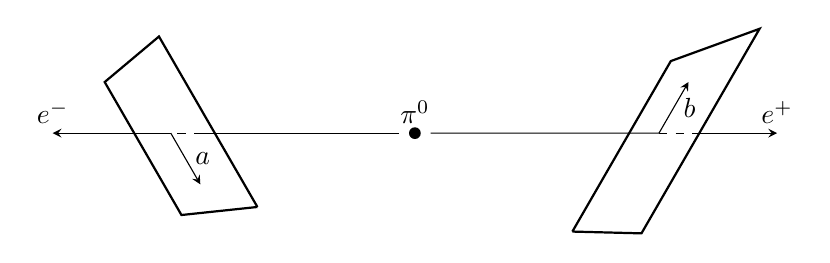
\begin{tikzpicture}
\pgfmathsetmacro{\anga}{60}
\pgfmathsetmacro{\angb}{180-\anga}
\pgfmathsetmacro{\a}{2}
\pgfmathsetmacro{\b}{1.25}
\pgfmathsetmacro{\c}{1.2}
\pgfmathsetmacro{\d}{3}
\draw[-stealth] (0.2,0) -- (3.1,0) --++ (\anga:0.75) node[pos=0.5,right]{$\kvec{b}$};
\draw[dashed](3.1,0)--++(0.5,0);
\draw[-stealth] (3.6,0) -- (4.6,0) node[above]{$e^{+}$};
\draw[] (-0.2,0) -- (-2.7,0);
\draw[dashed] (-2.7,0) -- (-3.1,0) coordinate(kl);
\draw[-stealth] (kl) --++ (\angb:-0.75) node[pos=0.5, right]{$\kvec{a}$};
\draw[-stealth] (kl) --++ (-1.5,0) node[above]{$e^{-}$};
\draw[] (0,0) node[circle, inner sep=1.5pt, fill=black]{} node[above]{$\pi^{0}$};
\draw[thick] (\a,-\b) coordinate(s) --++ (\anga:2*\b) --++ (20:\c) --++ (\anga:-\d) -- (s);
\draw[thick] (-\a,-0.75*\b) coordinate(ss) --++ (\angb:2*\b) --++ (-140:0.75*\c) --++ (\angb:-0.65*\d) -- (ss);
\end{tikzpicture}
\caption{آئنشٹائن، پوڈلسکی و  روزن  تضاد کا بل  انداز۔کاشف آزادانہ طور پر \عددی{\kvec{a}} اور \عددی{\kvec{b}} رخ سمت بند ہیں۔}
\label{شکل_بکھراو_بل_انداز}
\end{figure}


بل نے آئنساٹائن، پڈولسکی اور روزن بوہم تجربہ کو عمومی بنانے کی بات کی الیکٹران اور پوزیٹران کاشف کو ایک ہی رخ رکھنے کی بجائے بل نے انہیں علیحدہ علیحدہ زاویوں پر رکھنے کی اجازت دی۔ پہلا کاشف اکائی سمتیہ \عددی{a}  کے رخ الیکٹران چکر کا جز ناپتا ہے جبکہ دوسرا \عددی{b} کے رخ پوزیٹران کے چکر کا حصہ ناپتا ہے   (شکل \حوالہ{شکل_بکھراو_بل_انداز})۔ ہم اپنی آسانی کے لیئے چکر کو \عددی{\hslash/2} کی اکائیوں میں ناپتے ہیں یوں کاشف کے رخ ہم میدان کی قیمت \عددی{+1} اور خلاف میدان کی قیمت \عددی{-1} ناپی جائے گی۔ کئی \عددی{\pi^0} تنزل کے نتائج درج ذیل جدول میں پیش کئے گئے نتائج کی طرح ہوسکتے ہیں۔
\begin{table}[h!]
\begin{center}
\begin{tabular}{|c c c|}
\hline
الیکٹران & پوزیٹران &حاصل  ضرب \\
$+1$ & $-1$ & $-1$ \\
$+1$ & $+1$ & $+1$ \\
$-1$ & $+1$ & $-1$ \\
$+1$ & $-1$ & $-1$ \\
$-1$ & $-1$ & $+1$ \\
$\vdots$ & $\vdots$ & $\vdots$ \\
\hline
\end{tabular}
\end{center}
\end{table}
کاشف کے رخوں کی کسی ایک جوڑی کے لیئے بل نے چکر کے حاصلِ ضرب کی اوسط قیمت تلاش کی جسے ہم \عددی{P(a,b)} لکھتے ہیں۔ متوازی کاشفوں کی صورت میں \عددی{b=a} ہوگا جو ہمیں اصل آئنسٹائن، پڈلسکی، روزن اور بوہم تجربہ کے نتائج دیگا ایسی صورت میں ایک ہم میدان اور دوسرا خلاف میدان ہوگا لحاظہ ان کا حاصل ضرب ہر صورت \عددی{-1} ہوگا اور یوں اوسط کی قیمت بھی یہی ہوگی
\begin{align}
	P(a, a) = -1
\end{align}
اسی طرح اگر کاشف زد متوازی ہوں تب \عددی{b=-a} اور ہر حاصل ضرب \عددی{+1} لحآظہ درج ذیل ہوگا
\begin{align}
	P(a, -a) = +1
\end{align}
اختیاری سمت بندی کے لیئے کواانٹم میکانیات درج ذیل پیشاً گوئی کرتی ہے
\begin{align}
	P(a, b) = -a\cdot b
\end{align}
\حوالہء{سوال \num{4.50}} دیکھیں۔ بل نے دریافت کیا کہ یہ نتیجہ کسی بھی درپردہ متغیر نظریہ کا ہم اہنگ نہیں ہوسکتا ہے۔

اسکا دلیل حیرت کن حد تک سادہ ہے فرض کریں الیکٹران پوزیٹران نظام کے مکمل حال کو کوئی درپردہ متغیر یا متغیرات \عددی{\lambda} ظاہر کرتا ہے۔ ایک پائیون تنزل سے دوسرے پائیون تنزل تک \عددی{\lambda} کی تبدیلی کو نہ ہم سمجھتے اور نہ ہی قابو کرتے ہیں۔ ساتھ ہی فرض کرتے ہیں کہ الیکٹران کی پیمائش پر پوزیٹران کاشف کی سمت بندی \عددی{b} کا کوئی اثر نہیں پایا جاتا ہے یاد رہے کہ تجربہ کرنے والا الیکٹران کی پیمائش کے بعد پوزیٹران کاشف کا رخ منتخب کرسکتا ہے۔ ایسی صورت میں چونکہ پوزیٹران کاشف کا رخ منتخب کرنے سے پہلے ہی الیکٹران کی پیمائش کی جا چکی ہوگی لحاظہ اس پر بھی کی سمت کا کوئی اثر نہیں ہوسکتا ہے۔ یہ اصول مقامیت کا مفروضہ ہے یوں الیکٹران کی پیمائش کوئی تفاعل \عددی{A(a, \lambda)} اور پوزیٹران کی پیمائش کوئی دوسرا تفاعل \عددی{B(b, \lambda)} دیگا۔ ان تفاعلات کی قیمتیں صرف \عددی{\pm1} ہوسکتی ہیں
\begin{align}
	A(a, \lambda) = \pm1; && B(b, \lambda) = \pm1
\end{align}
جب کاشف متوازی ہوں تب تمام \عددی{\lambda} کے لیئے درج ذیل ہوگا 
\begin{align}
	A(a, \lambda) = -B(a, \lambda)
\end{align}
اب پیمائشوں کی حاصل ضرب کی اوسط قیمت درج ذیل ہوگی جہاں \عددی{\rho(\lambda)} درپردہ متغیر کی کثافت احتمال ہے
\begin{align}
	P(a, b) = \int\rho(\lambda)A(a, \lambda)B(b, \lambda)\dif\lambda
\end{align}
کسی بھی کثافت کا احتمال کے لیئے یہ غیر منفی ہوگا اور معمولزنی شرط \عددی{\int\rho(\lambda)\dif\lambda=1} کو متمعن کرے گا تاہم اس کے علاوہ ہم \عددی{\rho(\lambda)} کے بارے میں کچھ بھی فرض نہیں کرتے ہیں درپردہ متغیر کے مختلف نظریات \عددی{\rho} کے لیئے کافی مختلف تفاعلات پیش کر سکتے ہیں۔ \حوالہء{مساوات \num{12.6}} کو استعمال کرتے ہوئے ہم \عددی{B} کو خارج کر سکتے ہیں۔
\begin{align}
	P(a, b) = -\int\rho(\lambda)A(a, \lambda)A(b, \lambda)\dif\lambda
\end{align}
اگر \عددی{c} کوئی تیسرا اکائی سمتیہ ہو ت بدرج ذیل ہوگا
\begin{align}
	P(a, b)-P(a, c) = -\int\rho(\lambda)\left[A(a, \lambda)A(b, \lambda)-A(a, \lambda)A(c, \lambda)\right]\dif\lambda
\end{align}
اور چونکہ \عددی{[A(b, \lambda)]^2=1} ہے لحاظہپ درج ذیل ہوگا 
\begin{align}
	P(a, b)-P(a, c) =-\int\rho(\lambda)\left[1-A(b, \lambda)A(c, \lambda)\right]A(a, \lambda)A(b, \lambda)\dif\lambda
\end{align}
تاہم \حوالہء{مساوات \num{12.5}} کے تحت \عددی{-1\leq[A(a, \lambda)A(b, \lambda)]\leq+1} مزید \عددی{\rho(\lambda)[1-A(b, \lambda)A(c, \lambda)]\geq0} لحاظہ 
\begin{align}
	\abs{P(a, b)-P(a,c)}\leq\int\rho(\lambda)\left[1-A(b, \lambda)A(c, \lambda)\right]\dif\lambda
\end{align}
یا مختصراً درج ذیل ہوگا
\begin{align}
	\abs{P(a, b)-P(a, c)}\leq1+P(b, c)
\end{align}
یہ مشہور بل عدم مساوات ہے۔ \حوالہء{مساوات \num{12.5} اور \num{12.6}} کے علاوہ کوئی شرط عائد نہیں کی گئی ہے ہم نے درپردہ متغیرات کی تعداد یا خاصیت یا تقسیم \عددی{\rho} کے بارے میں کچھ بھی فرض نہیں کیا لحاظہ یہ عدم مساوات ہر مکامی درپردہ متغیر نظریہ کے لیئے کارامد ہوگا۔


\begin{figure}
\centering
\begin{tikzpicture}
\draw[-stealth] (0,0) -- (3,0) node[below]{$\kvec{a}$};
\draw[-stealth] (0,0) -- (0,3) node[left]{$\kvec{b}$};
\draw[-stealth] (0,0) --++ (45:2.5) node[above]{$\kvec{c}$};
\draw[] ([shift={(0:0.5)}]0,0) arc (0:45:0.5) node[pos=0.6,right]{$45^{o}$};
\draw[] ([shift={(45:0.75)}]0,0) arc (45:90:0.75) node[pos=0.5,shift={(67.5:0.3)}]{$45^{o}$};
\end{tikzpicture}
\caption{کاشف کو یوں سمت بند کیا گیا ہے کہ بل عدم مساوات کی کوانٹائی   خلاف ورزی   ظاہر ہو۔}
\label{شکل_بکھراو_بل_عدم_مساوات}
\end{figure}

لیکن ہم بہت آسانی ساے دیکھا ساکتے ہیں کہ کوانٹم میکانیات کی پیشاً گوئی \حوالہء{مساوات \num{12.4}} اور بل عدم مساوات ہم اہن نہیں ہیں۔ فرض کریں تینوں اکائی سمتیات ایک مستوی میں پائے جاتے ہوں اور \عددی{a} اور \عددی{b} کے ساتھ \عددی{c} کا زاویہ \عددی{45^\circ} ہو (شکل \حوالہ{شکل_بکھراو_بل_عدم_مساوات})۔ ایسی صورت میں کوانٹم میکانیات کہتی ہے کہ 
\begin{align*}
	P(a, b) = 0, && P(a, c) = P(b, c) = -\num{0.707}
\end{align*}
جبکہ بل عدم مساوات کہتی ہے کہ
\begin{align*}
	\num{0.707}\nleq1-\num{0.707} = \num{0.293}
\end{align*}
جہ ایک دوسرے کے غیر ہم اہنگ نتائج ہیں یوں بل کی ترمیم سے آئنسٹائن، پڈولسکی اور روزن تضاد ایک ایسی بات ثآبت کرتا ہے جو اس کے مصنفین تصور بھی نہیں کر سکتے تھے۔ اگر وہ درست ہوں تب نہ صرف کوانٹم میاکانیا نہ مکمل ہے بلکہ یہ مکلمل طور پر غلط ہے اس کے بر عکس اگر کوانٹم میکانیا درست ہے تب کوئی درپردہ متغیر نظریہ ہمیں اس غیر مکامیت سے نجات نہیں دو سکتی جسے آئنسٹائن مضائقہ خیز سمجھتا تھا۔	 مزید اب ہم بہت سادی تجربہ سے اس مسئلے کو دفنا سکتے ہیں۔

بل عدم مساوات کو پرکھنے کے لیئے ساٹھ اور ستر کی دیہائیوں میں کئی تجربات سرانجام دئے گئے جن میں ایسمیکٹ، گرینگیئر اور روجر کا کام قابلِ فخر ہے ہمیں یہاں انکے تجربہ کی تفصیل سے دلچسپی نہیں ہے۔ انہوں نے پائیون تمزل کی بجائے دو فوٹان جوہری انتقال استعمال کیا یہ خدشہ دور کرنمے کے لیئے کہ الیکٹران کاشف کی سمت بندی کو کسی طرح پوزیٹران کاشف جان پائے گا  فوٹان کی راوانگی کے بعد دونوں کی سمت بندی کی گئی۔نتائج کوانٹم میکانیات کی پیشاً گوئی کی عین مطابق تھے اور بل عدم مساوات کے غیر ہم اہنگ تھے۔

ستم ظریفی کی بات ہے کہ کوانٹم میکانیات کی تجرباتی تصدیق نے سائنسی برادری کو ہلا کر رکھ دیا۔ لیکن اس کی وجہ حقیقت پسند سوچ کا غلط ثابت ہونا نہیں تھا عموماً سائنسدان کب کے اس حقیقت کو مان چکے تھے اور جو ابھی بھی مانتے تھے انکے لیئے غیر مکامی درپردہ متغیر نظریات کا راستہ ابھی کھلا ہے چونکہ مثلا بل اطلاق ان پر نہیں ہوتا ہے۔ اصل سدمہ اس بات کا تھا کہ قدرت ازخود بنیادی طور پر غیر مکامی ہے۔ تفاعل موج کی فوراً انہدام کی صورت میں غیر مکامیت یا متماثل ذرات کے لیئے ضرورت تشاکلیت ہمیشہ تقلید پسند نظریہ کی خاصیت رہی ہے۔ تاہم ایسپیکٹ کے تجربہ سے قبل اُمید کی جاسکتی تھی کہ کوانٹم غیر مکامیت کسی طرح قائد و ضوابط کی غیر طبعی پیداوار تھی جس کے قابلِ کشف اثرات نہیں ہوسکتے ہیں اس اُمید کو بھول جائیں ہمیں فاصلہ پر یکدم عمل کے تصور کو دوبارہ دیکھنا ہوگا۔

\begin{figure}
\centering
\pgfmathsetmacro{\ra}{0.3}
\pgfmathsetmacro{\rb}{0.5}
\begin{tikzpicture}[declare function={fa(\t)=\ra*cos(\t); fb(\t)=\rb*sin(\t);}]
%\draw[] (0,0) circle (0.3cm and 0.5cm);
\draw[] plot[domain=120:420]({fa(\x)},{fb(\x)});
\draw[thick] ({fa(120)},{fb(120)})coordinate(bba) -- ({fa(420)},{fb(420)})coordinate(bbb)coordinate[pos=0.5](bbc);
\draw[thick](bba) to [out=90, in=90] (bbb);
\draw(bbc) to [out=90,in=45]++(0.3,0.3);
\draw(bbc) to [out=90,in=135]++(-0.3,0.3);
\draw[thin](bbc)--({fa(270)},{fb(270)});
\draw[] ({fa(35)},{fb(35)}) to [out=70,in=-160] ++ (0.2,0.2);
\draw[] ({fa(145)},{fb(145)}) to [out=110,in=-20] ++ (-0.2,0.2);
\draw[] ({fa(-45)},{fb(-45)}) to [out=-10,in=135] ++ (0.2,-0.2);
\draw[] ({fa(-135)},{fb(-135)}) to [out=-170,in=45] ++ (-0.2,-0.2);
\draw[] ({fa(0)},{fb(0)}) to [out=10,in=170] ++ (0.2,0);
\draw[] ({fa(180)},{fb(180)}) to [out=170,in=10] ++ (-0.2,0);
%
\draw[](-1,-1)--++(2,-1)node[pos=0.25,below left]{\RL{پردہ}} --++(0,4.5) --++ (-2,-0.5) -- cycle;
\draw[] (0,-1.25) node[circle, inner sep=1.5pt, fill= black]{} node[right]{$X$};
\draw[-stealth] (0,0.75) --++ (0,0.75) node[pos=0.65, right]{$\kvec{v}'$};
\draw[] (0,2) node [circle, inner sep=1.5pt, fill= black]{} node[right]{$Y$};
\draw[dashed] (-0.3,0.1) --++ (-5,0);
\draw[](-5.3,-1.3) rectangle++(-0.5,1);
\draw[thick] (-5.55,-0.3) --++ (0,0.2) coordinate(mm);
\draw[] (mm) to [out=45,in=-70] ++ (0,0.5);
\draw[] (mm) to [out=135,in=-90] ++ (0,0.5);
\fill[white] (-4.5,0.1) circle (0.3cm and 0.5cm);
\begin{scope}[xshift=-4.5cm,yshift=0.1cm, scale=0.3]
\draw[] plot[domain=120:420]({fa(\x)},{fb(\x)});
\draw[thick] ({fa(120)},{fb(120)})coordinate(bba) -- ({fa(420)},{fb(420)})coordinate(bbb)coordinate[pos=0.5](bbc);
\draw[thick](bba) to [out=90, in=90] (bbb);
\draw(bbc) to [out=90,in=45]++(0.3,0.3);
\draw(bbc) to [out=90,in=135]++(-0.3,0.3);
\draw[thin](bbc)--({fa(270)},{fb(270)});
\draw[] ({fa(35)},{fb(35)}) to [out=70,in=-160] ++ (0.2,0.2);
\draw[] ({fa(145)},{fb(145)}) to [out=110,in=-20] ++ (-0.2,0.2);
\draw[] ({fa(-45)},{fb(-45)}) to [out=-10,in=135] ++ (0.2,-0.2);
\draw[] ({fa(-135)},{fb(-135)}) to [out=-170,in=45] ++ (-0.2,-0.2);
\draw[] ({fa(0)},{fb(0)}) to [out=10,in=170] ++ (0.2,0);
\draw[] ({fa(180)},{fb(180)}) to [out=170,in=10] ++ (-0.2,0);
\end{scope}
\draw[-stealth] (-4.5,0.5) --++ (0,0.5) node[right]{$\kvec{v}$};
\draw[] (-4.5,-0.3) node[]{\RL{کیڑا}};
\end{tikzpicture}
\caption{پردہ پر کیڑے کا سایہ، روشنی کی رفتار \عددی{c} سے زیادہ رفتار \عددی{\kvec{v}'} سے  حرکت کرتا ہے بشرطیکہ  پردا  کافی دور ہو۔}
\label{شکل_بکھراو_موم_بتی}
\end{figure}

ماہر طبیعیات روشنی سے زیادہ تیز رفتار اثر و وسوخ کو کیوں برداشت نہیں کر سکتے ہیں؟ آخر کئی چیزیں روشنی سے زیادہ تیز رفتار سے حرکت کرتی ہے۔ ایک موم بتی کے سامنے چلتے ہوئے کیڑے کا سامنے دیوار پر ساے کی رفتار دیوار تک فاصلے کے راست متناسب ہوگی اصولاً آپ اس فاصلہ کو اتنا بڑھا سکتے ہیں کہ سایہ کی رفتار روشنی سے زیادہ ہو (شکل \حوالہ{شکل_بکھراو_موم_بتی})۔ تاہم دیوار پر کسی ایک نقطہ سے دوسرے نقطہ تک سایہ نہ کوئی توانائی منتقل کرسکتا ہے اور نہ ہی کوئی خبر پہنچا سکتا ہے۔ نقطہ \عددی{X} پر ایک شخص ایسا کوئی عمل نہیں کر سکتا جو یہاں سے گزرتے ہوئے ساے کے ذریعہ نقطہ \عددی{Y} پر اثر انداز ہو۔

%===============================

اس کے برعکس روشنی سے زیادہ تیز حرکت کرنے والے سببی اثر و وسوخ کے ناقبلِ قبول مضمرات ہو سکتے ہیں۔ خصوصی نظریہ اضافت میں ایسے جمودی چوکھٹ پائے جاتے ہیں جن میں اس طرح کا اشارہ وقت میں پیچھے جاسکے گا یعنی سبب سے پہلے اثر رونما ہوگا جس سے ناقابلِ قبول منتقی مسائل کھڑے ہوتے ہیں۔ مثلاً آپ اپنے نوزادہ دادا کو قتل کر سکتے ہیں۔ جو ظاہر ہے ایک بری بات ہے۔ اب سوال یہ کھڑا ہوتا ہے کہ آیہ روشنی سے تیز اثرات جن کیپیشاً گوئی کوانٹم میکانیات کرتی ہے اور جو ایسپیکٹ کے تجربہ میں کسف ہعتے ہیں ان معانوں میں سببی ہے یا یہ ساے کی حرکت کی طرح غیر حقیقی ہے جن پر فلسفیانہ اعترازات نہیں لگائے جا سکتے ہیں۔

آئیں تجربہ بل پر غور کریں کریں۔ کیا الیکٹران کی پیمائش کا پوزیٹران کی پیمائش پر اثر ہوگا  یقیناً ایسا ہوتا ہے ورنہ ہم مواد کے بیچ باہم رشتہ کی وضاحت پیش کرنے ساے قاصر ہوں گے۔ لیکن کیا الیکتران کی پیمائش پوزیٹران کی کسی مضصوص نتیجہ کا سبب ہے؟ الیکٹران کاشف پر بیٹھا شخص اپنی پیمائش کے ذریعہ پوزیٹران کاشف پر بیٹھے شخص کو اشارہ نہیں بھیج سکتا ہے چونکہ یہ اپنی پیمائش کے نتیجہ کو قابو نہیں کرتا یہ الیکٹران کو ہم میدان ہونے پر مجبور نہیں  کر سکتا ہے جیسا نقطہ \عددی{X} پر کیڑا کے ساے پر وہ شخص اثرانداز نہیں ہوسکتا، ہاں الیکٹران کاشف پر بیٹھا شخص فیصلہ کر سکتا ہے کہ وہ پیمائش کرے یا نہ کرے تاہم پوزیٹران کاشف پر بیٹھا شخص اپنی پیمائشی نتائج کو دیکھ کر یہ نہیں بتا سکتا کہ الیکٹران پر پیمائش کی گئی یانہیں دونوں کاشف کے نتائج پر علیحدہ علیحدہ غور کرنے سے مکمل بلاواستہ مواد دیکھنے کو ملتا ہے۔ صرف دونوں مواد کا ایک دوسرے کے ساتھ موازنہ کرنے سے ہمیں ان کے بیچ باہم رشتہ نظر آتا ہے کسی دوسرے جمودی چوکھٹ میں الیکٹران کی پیمائش سے قبل پوزیٹران کی پیمائش کی جائے گی لیکن اس کے باوجود اس سے کوئی منتقی تضاد پیدا نہیں ہوتا۔ دیکھا گیا باہم رشتہ اس پر منحصر نہیں کہ ہم کہیں الیکٹران کی پیمائش پوزیٹران کی پیمائش پر اثرانداز ہوتی ہے یا پوزیٹران کی پیمائش الیکٹران کی پیمائش پر اثرانداز ہوتی ہے۔ یہ ایک نہایت نازک اور خوبصورت اثر ہے جو بلا واستہ مواد کے بیچ باہم رشتہ کی صورت میں نظر آتا ہے۔

یوں ہمیں مختلف قسم کے اثرات کی بات کرنی ہوگی سببی قسم جو وصول کنندہ کی کسی طبعی خاصیت میں حقیقی تبدیلیاں پیدا کرتا ہو جنہیں صرف زیلی نظام پر تجرباتی پیمائش سے کشف کیا جا سکتا ہو اور آسمانی قسمپ جو توانائی یا معلومات کی ترسیل نہیں کرتا اور جس کے لیئے واحد ثبوت دو علیحدہ زیلی نظاموں کے مواد کے بیچ باہم رشتہ ہے۔ اس باہم رشتہ کو کسی بھی طرح کسی ایک زیلی نطام میں تجربات کے نتائج کو دیکھ کر کشف نہیں کیا جا سکتا ہے۔ سببی اثرات  رشنی کی رفتار سے تیز حرکت نہیں کر سکتے ہیں جبکہ آسمانی اثرات پر ایسی کوئی پابندی عائد نہیں۔ تفاعل نوج کی انہدام سے وابستہ اثرات مئخرالذکر قسم کی ہے جس کا روشنی سے تیز سفر کرنا حیران کن ضرور ہوسکتا ہے لیکن تباہ کن نہیں ہے۔
%========================

\حصہ{مسئلہ کلمیہ}
کوانٹم پیمائش عموماً تباہ کن ہوتے ہیں یعنی یہ پیمائش کردہ نظام کے حال کو تبدیل کرتا ہے۔ یہی تجربہ گاہ میں اصول عدم یقینیت کو یقینی بناتا ہے ہم کیوں اصل حال کی کئی متماثل نقل کلمیہ بنا کر اصل نظام کو چھوئے بغیر ان کی پیمائش نہیں کرتے ایسا کرنا ممکن نہیں ہے۔ اگر آپ کلمیہ بنانے والا ایسا آلا بنا پائیں تو کوانٹم میکانیات کو خداحافظ کہنا ہوگا۔

مثال کے طور پر آئنسٹائن، پوڈلسکی، روزن اور بوہم تجربہ کے ذریعہ روشنی سے تیز رفتار پر خبر بھیجنا ممکن ہوگا فرض کریں پوزیٹران کاشف چلانے ولا شخص ہاں یا نہیں کی خبر ترسیل کرتا ہے۔ خبر ہاں ہونے کی صورت میں بھیجنے والا پوزیٹران کا \عددی{S_z} ناپتا ہے یہ جاننے کی ضرورت نہیں کہ پیمائشی نتیجہ کیا ہے صرف اتنا جاننا ضروری ہے کہ پیمائش کی گئی ہے یوں الیکٹران کسی غیر مبہم حال \عددی{\uparrow} یا \عددی{\downarrow} میں ہوگا جسکا جاننا غیر اہم ہے۔ خبر وصول کرنے والا جلدی سے الیکٹران کی دس لاکھ کلمیہ تیار کر کے ہر ایک کی \عددی{S_z} ناپتا ہے اگر تمام کا ایک ہی جواب ہو کونسا جواب یہ جاننا ضروری نہیں ہم یقین سے کہہ سکیں گے کہ الیکٹران کی پیمائش کی گئی لحاظہ خبر ہاں ہوگی۔ اس کے برعکس اگر نصف الیکٹران ہم میدان اور نصف خلاف میدان ہوں تب یقیناً الیکٹران کی پیمائش نہیں کی گئی اور خبر نہیں ہوگا۔

لیکن سن \num{1982} ووٹرز، زورک اور ڈائکس نے ثابت کیا کہ ایسا مشین تیار نہیں کیا جا سکتا ہے جو کوانٹم متماثل ذرات پیدا کرتا ہو ہم چاہیں گے کہ یہ مشین حال \عددی{\mid\psi\rangle} میں ایک ذرہ جس کا نقل بنانا مقصود ہو اور حال \عددی{\mid X\rangle} میں ایک اضافی ذرہ لی کر  حال \عددی{\mid\psi\rangle} میں دو ذرات  اصل اور نقل دیتا ہو 
\begin{align}
	\mid\psi\rangle\mid X\rangle\to\mid\psi\rangle\mid\psi\rangle
\end{align}
فرض کریں ہم ایسا مشین بنانے میں کامیاب ہوتے ہیں جو حال \عددی{\mid\psi_1\rangle} کا کلمہ تیار کرتا ہو 
\begin{align}
	\mid\psi_1\rangle\mid X\rangle\to\mid\psi_1\rangle\mid\psi_1\rangle
\end{align}
اور \عددی{\mid\psi_2\rangle} پر بھی کام کرنے کے قابل ہو
\begin{align}
	\mid\psi_2\rangle\mid X\rangle\to\mid\psi_2\rangle\mid\psi_2\rangle
\end{align}
مثال کے طوور پر اگر ذرہ ایک الیکٹران ہو تب \عددی{\mid\psi_1\rangle} اور \عددی{\mid\psi_2\rangle} ہم میدان اور خلاف میدان ہو سکتے ہیں۔ یہاں تک کوئی مسئلہ پیدا نہیں ہوتا یہ دیکھان ہوگا کہ ان کا خطی جوڑ \عددی{\mid\psi\rangle=\alpha\mid\psi_1\rangle+\beta\mid\psi_2\rangle} کی صورت میں کیا ہوگا؟ ظاہر ہے ایسی صورت میں درج ذیل ہوگا
\begin{align}
	\mid\psi\rangle\mid X\rangle\to\alpha\mid\psi_1\rangle\mid\psi_1\rangle+\beta\mid\psi_2\rangle\mid\psi_2\rangle
\end{align}
جو ہم نہیں چاہتے ہیں۔ ہم درج ذیل چاہتے ہیں  
\begin{align}
	\mid\psi\rangle\mid X\rangle\to\mid\psi\rangle\mid\psi\rangle &= [\alpha\mid\psi_1\rangle+\beta\mid\psi_2\rangle][\alpha\mid\psi_1\rangle+\beta\mid\psi_2\rangle]\nonumber \\
	&= \alpha^2\mid\psi_1\rangle\mid\psi_1\rangle+\beta^2\mid\psi_2\rangle\mid\psi_2\rangle+\alpha\beta[\mid\psi_1\rangle\mid\psi_2\rangle+\mid\psi_2\rangle\mid\psi_1\rangle]
\end{align}
آپ ہم میدان الیکٹران اور خلاف میدان الیکٹران کے کلمہ بنانے کی مشین بنا سکتے ہیں لیکن وہ کسی بھی اہم خطی جوڑ کی صورت میں ناکامی کا شکار ہوگا یہ بلکل ایسا ہوگا جیسا نقل بنانے کی مشین  افکی لکیروں اور انتسابی لکیروں کی نقل خوش اصلوبی سے کرتا ہو لیکن وتری لکیروں کو مکمل طور پر بگاڑتا ہو۔
%================

\حصہ{شروڈنگر کی بلّی}
کوانٹم میکانیات میں پیمائش کا عمل ایک شرارتی کردار ادا کرتا ہے جس میں عدم تعینیت غیر مکامیت تفاعل موج کا انہدام اور باقی تمام تصوراتی مشکلات رونما ہتی ہیں۔ پیمائش کی غیر موجودگی میں مساوات شروڈنگر کے تحت تفاعل موج قابلِ تعین طریقہ سے ارتقا کرتا ہے اور کوانٹم میکانیات کسی بھی سادہ نظریہ میدان کی طرح نظر آتا ہے جو کلاسیکی برقی حرکیات سے بہت سادہ ہوگا چونکہ دو میدان \عددی{E} اور \عددی{B} کی بجائے اس میں واحد ایک غیر سمتی \عددی{\psi} پایا جاتا ہے۔ یہ پیمائش کا عمل ہی ہے جو کوانٹم میکانیات میں عجیب و غریب کردار ادا کرتے ہوئے اس کو سمجھ سے باہر خواص سے نوازتا ہے۔ یہ پیمائش حقیقت میں ہے کیا؟ اسے گیگر طبعی عوامل سے کیا منفرد بناتا ہے اور ہم کس طرح جان سکتے ہیں کہ پیمائش کی گئی ہے؟

شعوڈنگر نے اپنے مشہر تضاد بلّی کے مفروضہ نے اس بنیادی سوال کو پیش کیا۔

ایک بلّی کو فولاد کے ایک بند ڈبے میں بند کیا جاتا ہے اس ڈبے میں ایک گائگر گنت کار اور کسی تاب کار مادہ کی اتنی چھوٹی مقدار رکھی جاتی ہے جس کا ایک گھنٹا میں صرف ایک جوہر کے تحلیل ہونے کا امکان ہو تاہم یہ بھی ممکن ہے کہ کوئی جوہر تحلیل نہ ہو تحلیل کی صورت میں گنت کار اس ڈبے میں ایک زہریلی گیس چھوڑتا ہے۔ ایک گھنٹا گزرنے کے بعد ہم کہہ سکتے ہیں کہ تحلیل نہ ہونے کی صورت میں یہ بلّی زندہ ہوگی۔ پہلی تحلیل اس کو زہر سے مار دیتی۔اس مکمل نظام کا تفاعل موج اس حقیقت کو ظاہر کرنے کے لیئے زندہ اور مردہ بلّی کے برابر حصوں پر مشتمل ہوگا۔

ایک گھنٹا کے بعد بلّی کا تفاعل موج درج ذیل روپ کا ہوگا
\begin{align}
	\psi=\frac{1}{\sqrt{2}}(\psi_{\text{\RL{زندہ}}}+\psi_{\text{\RL{مردہ}}})
\end{align}
یہ بلّی نہ تو زندہ اور نہ ہی مردہ ہے بلکہ پیمائش سے پہلے یہ ان دونوں کا ایک خطی جوڑ ہوگا یہاں کھڑکی سے اندر دیکھ کر بلّی کا حال جاننے کو پیمائش تصور کیا جائے گا۔ آپ کا دیکھنمے کا عمل بلّی کو زندہ یا مردہ ہونے پر مجبور کرتا ہے ایسی صورت میں اگر بلّی مردہ پائی جائے تو یقیناً اس کے زمہدار آپ ہی ہیں چونکہ آپ نے کھڑکی سے دیکھ کر اسے قتل کیا۔

شروڈنگر اس تمام کو ایک بکواس سے زیادہ نہیں سمجھتا تھا اور میرے خیال سے زیادہ تر ماہرِ طبیعیات ان  کے ساتھ متفق ہیں۔ کلاں بین اجسام کا دو مختلف حالات کی ایک خطی جوڑ کی صورت میں ہونے کا تصور بے معنی ہے۔ ایک الیکٹران تو ہم میدان اور خلاف میدان کے ایک خطی جوڑ کی صورت میں ہو سکتا ہے لیکن ایک بلّی زندہ اور مردہ حالات کے ایک خطی جوڑ کی صورت میں نہیں ہوسکتی ہے۔ اس کو کوانٹم میکانیات کی تقلید پسند تشریح کے ساتھ کس طرح ہم اہنگ بنایا جا سکتا ہے۔

شماریاتی مفہوم کے لحاظ سے مقبول ترین جواب یہ ہے کہ گنت کار کی گنتی پیمائش ہوگی نا کہ کھڑکی میں سے انسانی مشاہدہ پیمائش سے مراد وہ عمل ہے جو کلاں بین نظام پر اثر انداز ہو جو یہاں گنت کار ہے۔ پیمائش کا عمل اس لمحہ پر رونما ہوگا جب خردبین نظام جسے کوانٹم میکانیات کے قوانین بیان کرتا ہے کلاں بین نظام جسے کلاسیکی میکانیات کے قواعد بیان کرتے ہیں کے ساتھ اس طرح باہم عمل کرے جس سے دائمی تبدیلی رونما ہو۔ کلاں بین نظام ازخود منفرد حالات کی ایک خطی جوڑ کا مکین نہیں ہوسکتا ہے۔
\حصہ{کوانٹم زینو تضاد}
اس عجیب قصہ کی اہم ترین خاصیت تفاعل موج کا انہدام ہے۔ ایک پیمائش کے فوراً بعد دوسری پیمائش سے اسی نتیجہ کے حصول کی خاطر خالصتاً نظریاتی بنیادوں پر اسے متعارف کیا گیا تھا یقیناً اس دو رس  اصول موضوعہ کے قابلِ مشاہدہ اثرات بھی ہوں گے۔ مسرا اور سدرشان نے سن \num{1977} میں تفاعلی موج کی انہدام کا ایک ڈرامائی تجرباتی مظاہرہ تجویز کیا جسے انہوں نے کوانٹم زینو اثر کا نام دیا۔ ان کا تصور یہ تھا کہ ایک غیر مستحکم نظام مثلا ہیجان حال میں ایک جوہر کو بار بار پیمائشی عمل سے گزارا جائے۔ ہر ایک مشاہدہ تفاعل موج کو منہدم کر کے گھڑی کو دوبارہ صفر وسے چالو کرے گا اور یوں زیریں حال میں متوقے انتقال کو غیر معائنہ مدد تک روکا جاسکتا ہے۔

فرض کریں ایک نظام ہیجان حال \عددی{\psi_2} سے آغاز کرترا ہے اور زمینی حال \عددی{\psi_1} میں منتقلی کے لیئے اس کا قدرتی عرصہ حیات \عددی{\tau} ہے۔ عام طور پر \عددی{\tau} سے کافی کم وقتوں کے لیئے انتقالی احتمال وقت \عددی{t} کا راست متناسب ہوگا \حوالہء{مساوات \num{9.42}} دیکھیں چونکہ انتقالی شرح \عددی{1/\tau} ہے لحاظہ درج ذیل ہوگا 
\begin{align}
	P_{2\to1}=\frac{t}{\tau}
\end{align}
وقت \عددی{t} پر پیمائش کرنے کی صورت میں بالائی حال میں نظام ہونے کا احتمال درج ذیل ہوگا
\begin{align}
	P_2(t)=1-\frac{t}{\tau}
\end{align}
درض کریں ہم دیکھتے ہیں کے نظام بالائی حال میں ہی ہے ایسی صورت میں تفاعل موج واپس \عددی{\psi_2} پر منحدن ہوگا اور پورا عمل ایک بار نئے سرے سے دوبارہ شروع ہوگا۔ اگر ہم وقت \عددی{2t} پر دوسری پیمائش کریں تب بالائی حال میں نظام ہونے کا احتمال درج ذیل ہوگا 
\begin{align}
	\left(1-\frac{t}{\tau}\right)^2\approx1-\frac{2t}{\tau}
\end{align}
جو وہی ہے جو اس صورت ہوتا اگر ہم پہلی پیمائش کرتے ہی نہیں سادہ سوچ کے تحت ایسا ہی ہونا چاہیئے تھا۔ اگر ایسا ہی ہوتا تب نظام کا بار بار مشاہدہ کرنے سے کوئی فرق نہیں پڑتا اور نہ یی کوانٹم زینو اثر پیدا ہوتا تاہم بہت قلیل وقت کی صورت میں انتقالی احتمال وقت \عددی{t} کے بجائے \عددی{t^2} کا راست متانسب ہوگا \حوالہء{\num{9.39}} دیکھیں
\begin{align}
	P_{2\to1}=\alpha t^2
\end{align}
ایسی صورت میں دو پیمائشوں کے بعد بھی نظام کا بالائی حال میں ہونے کا احتمال درج ذیل ہوگا
\begin{align}
	\left(1-\alpha t^2\right)^2\approx 1-2\alpha t^2
\end{align}
جبکہ پہلی پیمائش نہ کرنے کی صورت میں اب احتمال درج ذیل ہوتا
\begin{align}
	1-\alpha(2t)^2\approx1-4\alpha t^2
\end{align}
آپ دیکھ سکتے ہیں کہ وقت \عددی{t} گزرنے کے بعد نظام کے مشاہدہ کی بنا زیریں حال میں منتقلی کا احتمال کم ہوا ہے۔

یقیناً \عددی{t=0} سے لیکر \عددی{t=T} تک \عددی{n} برابر وقفہ \عددی{T/n, 2T/n, 3T/n, \dots, T} پر نظام کا مشاہدہ کرنے کی وجہ سے اس دورانیہ کے آخر میں بھی نظام بالائی حال میں پائے جانے کا احتمال درج ذیل ہوگا
\begin{align}
	\left(1-\alpha(T/n)^2\right)^n\approx1-\frac{\alpha}{n}T^2
\end{align}
جو \عددی{n\to\infty} کی حد میں \عددی{1} تک پہنچتا ہے ایک غیر مستحکم نظام جس کا مسلسل مشاہدہ کیا جائے کبھی بھی تحویل نہیں ہوگا بعض مصنفین اس ماخوز سے اتفاق نہیں کرتے اور ان کے نزدیک یہ تفاعل موج کے انہدام غیر درست ہونے کا ثبوت ہے۔ تاہم ان کے سدلائل مشاہدہ کے مفہوم کی غلط تشریح پر مبنی ہے اگر بلبلا خانہ میں ایک ذرہ کی راہ کو مسلسل مشاہدہ کرار دے دیا جائے تب یہ بلکل درست ہوں گے چونکہ ایسی ذرات یقیناً تحویل ہوتے ہیں اور ان کا عرصہ حیات پرکاشف کا قابلِ پیمائش اثر نہیں پایا جاتا ہے تاہم ایسا ذرہ خانہ کے اندر جوہروں کے ساتھ خاد و خال  باہم عمل کرتا ہے جبکہ کوانٹم زینو اثر کے لیئے ضروری ہے کہ یکِ بعد دیگر پیمائشوں کے بیچ وقفہ اتنا کم ہو کہ نظام کو \عددی{t^2} خطہ میں پکڑا جائے۔

ہم دیکھتے ہیں کہ خود با خود انتقل کی صورت میں یہ تجربہ عملاً ممکن نہیں ہے۔ تاہم پیدا کردہ انتقال کی صورت میں نتائج کا نظریاتی پیشاً گوئی کے ساتھ مکمل اتفاق پایا جات ہے۔ بدقسمتی سے یہ تجربہ تفاعل موج کی انہدام کا ختمی ثبوت پیش نہیں کرسکتا ہے اس مشاہدہ کے دیگر وجوہات بھی دئے جاسکتے ہیں۔ 

میں نے اس کتاب میں ایک ہم اہہنگ اور بلا تضاد کہانی پیش کرنے کی کوشش کی ہے تفاعل موج \عددی{\psi} کسی ذرہ یا نظام کے حال کو ظاہر کرتا ہے۔ عمومی طور پر ای کذرہ کسی مخصوص حرکی خاصیت مثلاً مکام معیارِ حرکت توانائی زاویائی معیارِ حرکت وغیرہ کا حامل نہیں ہوتا اس وقت تک  جب پیمائشی عمل مداخلت نہ کرے کسی ایک تجربہ میں حاصل ایک مخصوص قیمت کا احتمال \عددی{\psi} کی شماریاتی مفہوم تعین کرتا ہے۔ پیمائشی عمل سے تفاعل موج منحدم ہوتا ہے جس کی بنا فوراً دوسری پیمائش لاظماً وہی نتیجہ دیگی۔ اگرچہ دیگر تشریحات مثلاً غیر مکامی درپردہ متغیر نظریات متعدد کائنات کا تصور بلا تضاد تاریخیں سگرہ نمونے وغیرہ بھی پائے جاتے ہیں لیکن میں یقین کرتا ہوں کہ یہ سب سے سادہ ہے جس سے عموماً ماہرِ طبیعیات اتفاق کرتے ہیں۔ یہ ہر تجربہ سے کامیابی سے ابھرا ہے تاہم یہ کہانی کا اختتام نہیں ہے ہمیں پیمائشی عمل کے بارے میں اور انہدام کے طریقے کار کے بارے میں بہت کچھ جاننا ہے عین ممکن ہے کہ آنے والے نسلیں زیادہ پیچیدا نظریہ جانتے ہوئے سوچتے ہوں کہ ہم اتنا سادہ کیسے ہوسکتے تھے۔

